\begin{enumerate}

\item {\bf (8 pts.)}
Design a digital circuit to debounce a pushbutton.  Your circuit
will have one input $X$ (see Figure~\ref{fig:pushbutton}) and
one (debounced) output $Z$. Your circuit will run off a 1MHz clock.  
The signal bouncing lasts at most 10mS.  You are to take 16 samples 
over a 10mS interval.  If all the samples agree then $Z$ should
equal the unanimous values.  If the samples disagree with one
another (as they will during a bounce) then $Z$ should remain
unchanged (stay at its previous value).  That is, the output of 
the debouncer should not change until there is compelling evidence to
in the form of complete and consistent disagreement to the current
output.

\item{\bf (16 pts.)} Design a digital circuit to keep track of the
number of net detents turned through on a rotary encoder.  The circuit
is to add CW rotation and subtract CCW rotations.  The count value
saturates at -128 or +127 as described in the 4-bit saturation
adder on page~\pageref{page:saturation}.

\begin{tabular}{|l|p{3.5in}|} \hline
Nomenclature:  & Encoder counter         \\ \hline
Data Input:    & none         \\ \hline
Data Output:   & 8-bit 2's complement   \\ \hline
Control:       & none           \\ \hline
Status:        & 1-bit busy                                   \\ \hline
Physical Input:& rotary encoder knob        \\ \hline
Physical Output:& none          \\ \hline
Others:        &            \\ \hline
Behavior:      & When the knob is turn from one detent to the next in
a CW direction the output should count up by 1.  When the knob is moved
through a full detent in the CCW direction the count should go down
by 1.  While the encoder is between detents the busy output
should equal 1. \\ \hline
\end{tabular}

Show your datapath and control, define the CW and write the binary control
word for each state.

\item{\bf (8 pts.)} Build a circuit which outputs the control sequence
to a stepper motor.

\item{\bf (32 pts.)} Build a digital stopwatch.

\begin{tabular}{|l|p{3.5in}|} \hline
Nomenclature:  & Stopwatch         \\ \hline
Data Input:    & none         \\ \hline
Data Output:   & 3 7-bit 7-segment values (unit, ten, min)   \\ \hline
Control:       & left, right           \\ \hline
Status:        & 1-bit BLINK                         \\ \hline
Physical Input:& none        \\ \hline
Physical Output:& none          \\ \hline
Others:        &            \\ \hline
Behavior:      & Keep track of elapsed time. \\ \hline
\end{tabular}

The stopwatch will have 2 bits of input provided by the
push buttons called left and right.  Your circuit will also have as 
input a 12Mhz ($12{\rm x}10^6$ hz) clock signal.   The output of the stop 
watch will be displayed on three seven segment displays.  Two 
displays will show seconds and one will show minutes.   The signal
BLINK is connected to an LED (or to the 7-segment display decimal points)
to indicate when the main TIMER is running.  The overall
architecture of the stopwatch is shown in Figure~\ref{fig:stopwatch_dp}.

\begin{figure}[ht]
\center{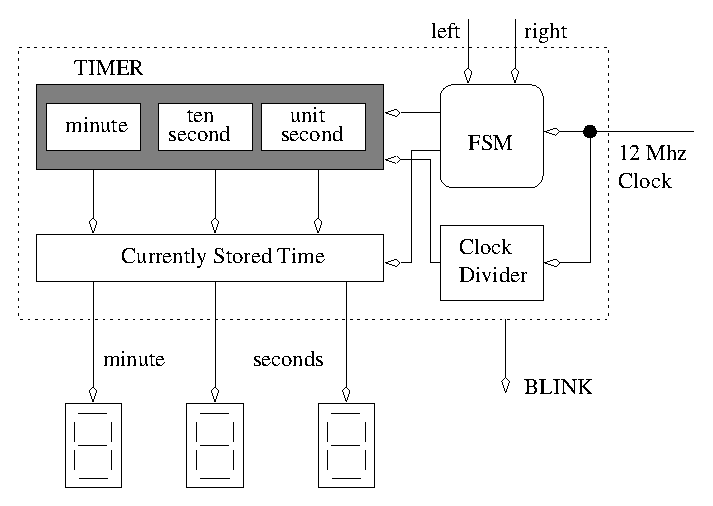
\includegraphics{./FigHw10/Prob10-4}}
\caption{The high level architecture of the stopwatch.}
\label{fig:stopwatch_dp}
\end{figure}

From Figure~\ref{fig:stopwatch_dp} it can be seen that TIMERs
value is sent through a register called Currently Stored Time.
This allows the TIMER to run independent of the displayed time.
This is useful for example, when a runner wants to know how long 
a particular lap took to complete without loosing track of the 
total time to run all the laps.
This is typically called the lap state of a stopwatch.  From the 
users perspective the stopwatch will have four additional
states.  stop, run,  pause and reset.  Each state defines the
behavior of the TIMER, BLINK and Currently Store Time as described
in the following table

\begin{tabular}{l||l|l|l}
STATE	&	TIMER	& Currently Stored Time	& BLINK	\\ \hline \hline
STOP	&	stopped	&	hold		& off	\\ \hline
RUN	&	running	&	load		& blink	\\ \hline
LAP	&	running &	hold		& blink	\\ \hline
PAUSE	& 	stop	& 	hold		& off	\\ \hline
RESET	& reset to 0	& reset to 0		& off	\\ 
\end{tabular}

The user moves between the states by pressing the buttons
as shown in Figure~\ref{fig:stopwatch_fsm}.
button while in each of the five states.  Please note, while 
similar to the final state diagram, the state diagram shown in 
Figure~\ref{fig:stopwatch_fsm} will not work in the final circuit
because the user will probably hold down the buttons for more 
than a single clock cycles.  See page~\pageref{page:push_dp}
for more details.

\begin{figure}[ht]
\center{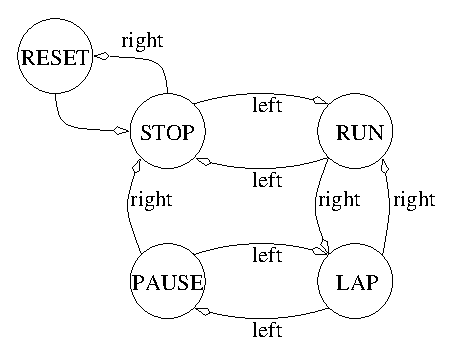
\includegraphics{./FigHw10/Prob10-4b}}
\caption{The users view of the stopwatch FSM.}
\label{fig:stopwatch_fsm}
\end{figure}

There are some major datapath elements which must be addressed
before the design is complete.  the following are some suggestions
to focus your thinking.
\begin{enumerate}
\item Generate a 1 Hz signal to feed into the timer counters
and the BLINK signal.
\item Build a mod 10 counter for unit second and minute.
\item Build a mod 6 counter for the tens of second counter.
\item Use control signals to tell the counter when to count
up.  Do not AND together control signals with the clock.
\end{enumerate}

Turn in; an algorithm
the datapath and control unit,
the control word table,
the memory input equations, and
output equations.
The control unit is to be implemented using a ones hot encoding.


\item{\bf (32 pts.)} Create a circuit that displays a fancy light 
pattern that is "programmed" in by the user and then displayed
automatically by the digital circuit.  The fancy lights circuit
has an 8-bit data output on which are arranged 8 active high LEDs.
The circuit also has two 7-bit outputs directed to 7-segment
displays.  In addition, the circuit has an 8-bit DIP switch and 2 
push buttons labeled EVENT and MODE.  There are two modes that the 
circuit operates in, program and recall.

In program mode an LED lights up when its corresponding DIP switch
is set to 1.   The 7-segment displays show the number of patterns
stored (out of a maximum of 256) in hexadecimal.  Initially
the hex displays will read 00.  When the user is satisfied with a 
particular arrangements of DIPs/LEDs they press the EVENT button.
The DIP switch value is stored in a RAM and the number of stored patterns
is incremented.  The user continues setting DIP switches and pressing
the EVENT button, creating a sequence of stored patters.  When the
user wants to stop entering patterns they press the MODE button and
the digital circuit enters the recall mode.

In recall mode the digital circuit cycles through the patterns
stored during the program mode.  The circuit should not cycle 
through any unused patterns.  The speed of the light animation
can be changed by pressing the EVENT button.  The speed should
cycle between 1 of 4 different values (1hz, 2hz, 4hz, and 8 hz).

You will need to make sure to include wait states in the FSM
in order to allow the user to remove their finger from the
button before completing a state transition.

Turn in; an algorithm
the datapath and control unit,
the control word table,
the memory input equations, and
output equations.
The control unit is to be implemented using a ones hot encoding.


\item {\bf(32 pts.)}
Build a sound manipulator using the stereo codec available on the
XESS corporation's XS40 or XSA-100 boards.  A stereo codec is a digital
devices which manipulates analog stereo audio waveforms.  A stereo audio signal
is composed of a left and right channel, meaning that the left and right
speakers (headphones) can produce different sounds.  When done well the
resulting effect is that of an actual live
musical performance.  The codec can convert between a stereo audio signal 
and a stream of 20-bit 2's complement values representing the amplitude
of the left or right channel.  The codec performs 44K such conversions 
per second.
 
In order to understand what is meant by the amplitude of the sound you first
must understand how sound is created by a speaker.  A speaker is a 2-wire
device whose main parts are the cone, diaphragm and electromagnet as 
shown in Figure~\ref{fig:speaker}.  The fundamental operation of a speaker 
is straight forward.  A voltage applied across the speaker leads causes
the electromagnet at the read of the speaker to move the cone.  Since
the cone is connected to the diaphragm then it moves. The mounting 
plate provides a solid mounting point for the diaphragm as well as a point
of attachment for the speaker.

\begin{figure}[ht]
\center{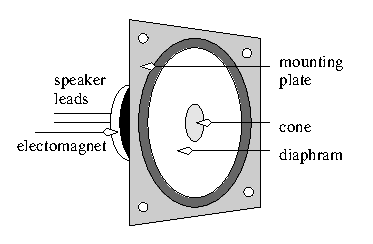
\includegraphics{./FigHw10/Prob10-6}}
\caption{The main parts of a speaker.}
\label{fig:speaker}
\end{figure}


A speaker converts electrical energy into sound as follows.  When a positive 
voltage is applied across the speaker leads the cone mechanically pushes 
the diaphragm out causing the air molecules in front of the  speaker to 
have a high air pressure.  When a negative voltage is 
applied across the leads of the speaker then the cone pulls the diaphragm 
inwards causing the air molecules in front of the speaker to have a low 
pressure.  Now imagine putting a 440Hz
sine wave across the leads of the speaker. The cone would be pushed and 
pulled in and out 440 times a second, creating pressure waves at 440Hz,
a perfect A note.  Note, a note created by a single sine wave is called 
a pure tone.

The codec can be thought of as digitizing the position of the speaker's
cone.  The codec assigns the resting state of the speaker the value
of 0 (or 0x00000 in 20-bit 2's complement).  The maximum extent of the cone
movement (+3V) is represented as 524,287 (or 0x7FFFF).  The minimum deflection of 
the cone (-3V) is represented -524,288 (or 0x80000).  
 The term codec is a combination of two words, COder
and DECoder.  This means that the codec is capable of coding an audio signal
into 20-bit 2's complement number and of simultaneously decoding 20-bit 2's
complement numbers into a pair of audio signals.   The processing of coding an analog
signal into a digital value is referred to as Analog to Digital Conversion or
ADC for short.  Likewise, the processing of decoding a digital value into an
analog signal is referred to as Digital to Analog Conversion or DAC for short.
To make working with the actual hardware codec easier you can obtain a firmware 
codec interface from your professor or from the XESS web site.  Figure~\ref{fig:codec} 
shows the codec\_intfc consisting of hardware and firmware 
building blocks. 

\begin{figure}[ht]
\center{ \scalebox{0.75}{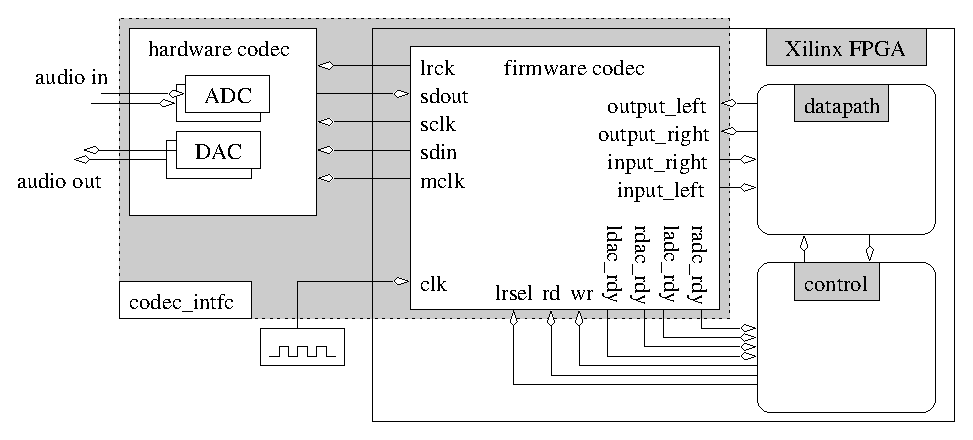
\includegraphics{./FigHw10/Prob10-6b}} }
\caption{A schematic showing the relationship between the stereo codec,
the Xilinx FPGA, the codec\_intfc and your digital circuit.}
\label{fig:codec}
\end{figure}


The firmware codec contains four 20-bit shift registers which perform 
serial to parallel and parallel to serial conversion.  If the hardware
codec used parallel communication it would require at least 80 pins
for its left and right channel and  data input and output.
  In order to minimize the pin count
of the chip the designers of the codec decided that all data transfers
to/from the codec should be serial.  While decreasing the pin count this
decision increases the amount of time required to fetch and store data
from/to the codec.  The hardware and firmware codecs communicate to
one another using the 5 signals shown.  No further mention of these 
signals will be made.  Of particular interest to you should any signal
which crosses the boundary of the codec\_intfc component.  These
signals are outlines in the description below.

\begin{tabular}{|l|p{3.5in}|} \hline
Nomenclature:  & codec\_intfc         \\ \hline
Data Input:    & input left,  input right  20-bit 2's complement   \\ \hline
Data Output:   & output left, output right 20-bit 2's complement   \\ \hline
Control:       & lrsel, rd, wr    \\ \hline
Status:        & radc\_rdy, ladc\_rdy, rdac\_rdy, ldac\_rdy     \\ \hline
Physical Input:& stereo audio input signal        \\ \hline
Physical Output:& stereo audio output signal        \\ \hline
Others:        & none					\\ \hline
Behavior:      & \scalebox{0.75}{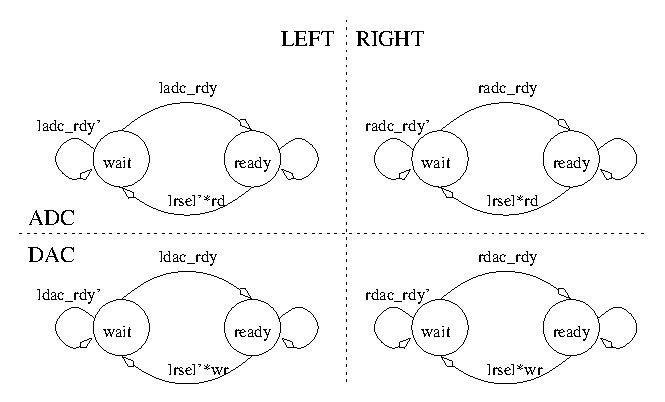
\includegraphics{./FigHw10/Prob10-6c}}	\\ \hline
\end{tabular}

The behavior of the stereo codec is driven by the four status signals
radc\_rdy (Right ADC ReaDY), ldac\_rdy (Left DAC ReaDY) etc.  These
status signals describe the state of four independent FSM inside the 
firmware codec.  For example, to generate a pure tone, the user 
would create a piece of hardware to monitor the ldac\_rdy and rdac\_rdy
signals.  When either went high the user would assert a 20-bit value
onto the corresponding output\_left or output\_right channel and then assert
the corresponding value on lrsel and then drive the write signal high.
One clock cycle latter the firmware codec will have latched the value
and consequently will lower the ldac\_rdy and rdac\_rdy signal.
In order to read a digitized sound the user 
would create a piece of hardware to monitor the ladc\_rdy and radc\_rdy
signals.  When either went high the user would read the 20-bit value
from the corresponding input\_left or input\_right channel.  Then the
circuit would select the corresponding value on lrsel signal and then 
drive the read signal high.  One clock cycle latter then firmware codec 
will have lowered the ladc\_rdy and radc\_rdy signal.


There are a variety of projects that can be realized using the stereo
codec.  Several are listed below.
\begin{enumerate}
\item Toggle between fade in and fade out on successive button presses.
\item Change output resolution from among 4 ranges (20,16,12,8)-bit 
based on two DIP switches.  That is, pass only the x most significant bits 
of the input to the output; where x is defined in the list above.  Set the
remaining 20-x bits of the output to zero.
\item Change DC-offset of sound data by $2^{17}, 2^{18}, 2^{19}, -2^{18}$ 
based on two DIP switches.  Make sure to use saturation addition, that
is do not let the result of your addition (or subtraction) roll over from a
positive number to a negative number (or vice versa).
\item Amplify (multiply) all signals by 0.25, 1.0, 1.5, 3.0 based on two
DIP switches.  Again, make sure to use a saturation adder.  
\item Amplify a signal based on its rate of change.  Use the following 
table as a rough guideline for the multiplicative factors; specifically 
use values which give close values for the frequencies but which work 
nicely in hardware.  Again make sure to use a saturation adder.

\begin{tabular}{l|l}
Frequency	&	Amplification \\ \hline \hline
 0-50    	&	    0.125     \\ \hline
 50-100  	&	    0.25      \\ \hline
100-200  	&	    0.5       \\ \hline
200-300  	&	    1.0       \\ \hline
400-800  	&	    2.0       \\ \hline
800-1600 	&	    4.0       \\ \hline
1600-3200	&	    8.0       \\ \hline
3200-6400	&	   16.0       \\ 
\end{tabular}

\item Record the peak-to-peak amplitude of the audio waveform on the bar LED.
\item Generate a square wave at 400 or 800Hz.  The frequency is selectable
with a DIP switch.  The waveform should have a large amplitude.
\item Multiple the digitized audio waveform values by a time varying function
called $\mathcal{F}$.  $\mathcal{F}$ should be a low frequency signal 
(around 1 to 4 Hz) whose value varies periodically between 0 and 1.
\end{enumerate}


\item {\bf (18 pts.)}
Build the VGA\_SYNCH component.
The VGA interface of the VGA\_SYNCH component has 5-bits of output
1-bits each for the red, green and
blue signals and 1 bit each of vertical and horizontal synch. The
input to the VGA\_SYNCH component consists of a 25.427095Mhz clock and a reset 
signal. The VGA\_SYNCH outputs the current pixel coordinates on the 
10-bit row and column outputs. The color that the user wants to 
display at the current pixel coordinates are fed into the 1-bit 
red, green, blue inputs.



\end{enumerate}
